\chapter{Caminhos Mínimos em Grafos}

O problema dos \textbf{caminhos mínimos} busca determinar o caminho de menor custo entre dois vértices em um grafo ponderado. 
Em outras palavras, dado um grafo $G = (V, E)$, com pesos $w(u,v)$ associados a cada aresta $(u,v)$, queremos encontrar o caminho de custo mínimo entre um vértice de origem e um vértice de destino.

Esse tipo de problema aparece em diversas situações práticas, como:

\begin{itemize}
    \item \textbf{Rotas de transporte:} determinar o trajeto mais curto entre duas cidades, ou o caminho mais rápido em um mapa (por exemplo, em sistemas de navegação como GPS ou Google Maps).
    \item \textbf{Redes de computadores:} definir rotas eficientes para o envio de pacotes de dados, minimizando o número de saltos ou o tempo total de transmissão.
    \item \textbf{Planejamento de tarefas e projetos:} encontrar a sequência de atividades que leva ao menor custo ou duração total, considerando dependências entre etapas.
\end{itemize}

Podemos classificar os problemas de caminhos mínimos em diferentes categorias, de acordo com o tipo de consulta desejada:

\begin{itemize}
    \item \textbf{Caminho mínimo a partir de uma origem} (\textit{single-source shortest path}): determinar o caminho de menor custo do vértice de origem $s$ a todos os demais vértices do grafo.
    \item \textbf{Caminho mínimo entre todos os pares de vértices} (\textit{all-pairs shortest paths}): determinar o menor custo entre cada par $(u, v)$ de vértices do grafo.
    \item \textbf{Caminho mínimo entre dois vértices específicos:} problema particular onde se deseja apenas o menor caminho entre $s$ e $t$.
\end{itemize}

Esses problemas têm grande importância em aplicações reais e servem de base para diversos outros algoritmos em teoria dos grafos e otimização.

\section{Conceitos Fundamentais}

Nesta seção apresentamos os conceitos básicos necessários para o estudo dos algoritmos de caminhos mínimos.

\subsection*{Grafos Ponderados}

Um \textbf{grafo ponderado} é um grafo $G = (V, E)$ no qual cada aresta $(u,v) \in E$ está associada a um número real $w(u,v)$, chamado \textbf{peso} ou \textbf{custo} da aresta. Esse peso pode representar, por exemplo, uma distância, um tempo de percurso, um custo financeiro ou uma capacidade de transmissão.

\[
w : E \rightarrow \mathbb{R}
\]

Dizemos que o grafo é \textbf{não direcionado} quando as arestas são bidirecionais (isto é, $(u,v)$ implica $(v,u)$ com o mesmo peso) e \textbf{direcionado} quando o sentido importa, isto é, $(u,v)$ e $(v,u)$ são arestas distintas, possivelmente com pesos diferentes.

\subsection*{Caminho, Custo e Distância Mínima}

Um \textbf{caminho} entre dois vértices $u$ e $v$ é uma sequência de vértices

\[
P = (v_0, v_1, v_2, \ldots, v_k)
\]
tal que $v_0 = u$, $v_k = v$ e $(v_{i-1}, v_i) \in E$ para todo $1 \le i \le k$.

O \textbf{custo do caminho} $P$ é definido como a soma dos pesos de suas arestas:

\[
w(P) = \sum_{i=1}^{k} w(v_{i-1}, v_i)
\]

A \textbf{distância mínima} (ou \textbf{caminho mínimo}) entre $u$ e $v$ é o menor custo entre todos os caminhos que ligam $u$ a $v$, denotada por $dist(u,v)$:

\[
dist(u,v) = \min_{P:u \leadsto v} w(P)
\]

\subsection*{Ciclos e Pesos Negativos}

Se todas as arestas possuem pesos não negativos, então a distância mínima entre dois vértices é sempre bem definida. 

Por outro lado, a presença de \textbf{pesos negativos} pode causar situações problemáticas: se existir um \textbf{ciclo de custo negativo} (ou seja, um caminho fechado cuja soma dos pesos é menor que zero), então é possível reduzir indefinidamente o custo de um caminho passando várias vezes por esse ciclo. Nesse caso, a noção de caminho mínimo deixa de fazer sentido, pois o custo pode tender a $-\infty$.

\subsection*{Propriedade de Otimalidade}

Uma propriedade fundamental dos caminhos mínimos é a chamada \textbf{propriedade de otimalidade}:

\begin{quote}
Qualquer subcaminho de um caminho mínimo também é um caminho mínimo entre os vértices que o delimitam.
\end{quote}

Essa propriedade é a base de todos os algoritmos de caminhos mínimos, pois garante que podemos construir soluções ótimas de forma incremental, a partir de subproblemas menores.

\section{O Princípio do Relaxamento}

A ideia central dos algoritmos de caminhos mínimos é o \textbf{relaxamento de arestas}.  
Cada vértice mantém uma \textbf{estimativa} do custo necessário para ser alcançado a partir da origem.  
O processo de relaxamento utiliza as arestas adjacentes para tentar \textbf{melhorar} essa estimativa.

\subsection*{Ideia Central}

Suponha que temos uma aresta $(u,v)$ com peso $w(u,v)$.  
Se o caminho passando por $u$ permite chegar a $v$ com um custo menor do que o atualmente conhecido, atualizamos a estimativa de distância de $v$.  
Formalmente, a operação de relaxamento é definida como:

\[
\text{se } dist[v] > dist[u] + w(u,v) \text{ então:}
\]
\[
\quad dist[v] := dist[u] + w(u,v)
\]
\[
\quad pai[v] := u
\]

Essa simples operação é o \textbf{coração} de todos os algoritmos de caminhos mínimos, desde o Dijkstra até o Bellman–Ford e Floyd–Warshall.

\subsection*{Propriedades}

\begin{itemize}
    \item As estimativas armazenadas em \texttt{dist[]} são sempre \textbf{maiores ou iguais} ao valor ótimo real da distância mínima.
    \item Quando nenhum relaxamento é mais possível, o algoritmo \textbf{convergiu}, isto é, todas as distâncias armazenadas são ótimas.
    \item O vetor \texttt{pai[]} armazena a estrutura da árvore de caminhos mínimos, permitindo reconstruir o caminho a partir da origem.
\end{itemize}

\subsection*{Exemplo Numérico}

Considere o grafo ponderado da Figura~\ref{fig:relaxamento-exemplo}, com quatro vértices e cinco arestas.  
Inicialmente, temos $dist[s] = 0$ e $dist[v] = \infty$ para todos os outros vértices.  
Ao relaxar as arestas que saem de $s$, obtemos novas estimativas de custo.  
Após algumas iterações, os valores de $dist[v]$ estabilizam, representando o menor custo possível a partir de $s$.

\begin{figure}[h]
 \centering
 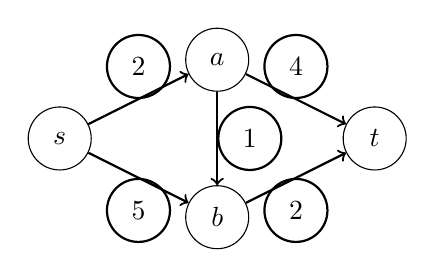
\begin{tikzpicture}[scale=1, every node/.style={circle, draw, minimum size=8mm}]
 \node (s) at (0,0) {$s$};
 \node (a) at (2,1) {$a$};
 \node (b) at (2,-1) {$b$};
 \node (t) at (4,0) {$t$};
 \draw[->, thick] (s) -- (a) node[midway, above] {2};
 \draw[->, thick] (s) -- (b) node[midway, below] {5};
 \draw[->, thick] (a) -- (b) node[midway, right] {1};
 \draw[->, thick] (a) -- (t) node[midway, above] {4};
 \draw[->, thick] (b) -- (t) node[midway, below] {2};
 \end{tikzpicture}
 \caption{Exemplo de relaxamento em um grafo ponderado.}
 \label{fig:relaxamento-exemplo}
\end{figure}

\subsection*{Implementação}

A seguir, apresentamos uma função simples que implementa o relaxamento de uma aresta:

\begin{lstlisting}[language=C, caption={Função de relaxamento de aresta.}]
void relax(int u, int v, int w) {
    if (dist[v] > dist[u] + w) {
        dist[v] = dist[u] + w;
        pai[v] = u;
    }
}
\end{lstlisting}

A operação \texttt{relax()} é usada repetidas vezes nos algoritmos de Dijkstra e Bellman–Ford, com diferentes estratégias de escolha e repetição das arestas a serem relaxadas.

\section{Estratégias de Aplicação do Relaxamento}

Os algoritmos de caminhos mínimos diferem essencialmente na forma como aplicam o \textbf{princípio do relaxamento}.  
Todos realizam a mesma operação básica — tentar melhorar as estimativas de custo usando as arestas —, mas adotam estratégias distintas quanto a:

\begin{itemize}
    \item \textbf{Quantas vezes} cada aresta é relaxada;
    \item \textbf{Em que ordem} as arestas são percorridas;
    \item \textbf{Quando parar} o processo de relaxamento.
\end{itemize}

Essas três decisões caracterizam o comportamento e a eficiência de cada algoritmo.  
O Dijkstra, por exemplo, escolhe sempre o vértice com a menor distância estimada e o considera \textit{finalizado}, enquanto o Bellman–Ford percorre todas as arestas várias vezes, até garantir que nenhuma melhora adicional é possível.

\begin{table}[h]
\centering
\caption{Estratégias de aplicação do relaxamento nos principais algoritmos.}
\begin{tabular}{|l|l|}
\hline
\textbf{Estratégia} & \textbf{Exemplo de Algoritmo} \\ \hline
Relaxa apenas as arestas que saem do vértice mais próximo ainda não processado & Dijkstra \\ \hline
Relaxa todas as arestas repetidamente, por até $|V|-1$ iterações & Bellman--Ford \\ \hline
\end{tabular}
\end{table}

Dessa forma, podemos ver o Dijkstra como uma abordagem \textbf{gananciosa} (\textit{greedy}), que escolhe sempre a melhor opção local, e o Bellman–Ford como uma abordagem \textbf{iterativa}, baseada em \textbf{programação dinâmica}, que refina gradualmente as estimativas até atingir a solução ótima.


\section{Algoritmo de Dijkstra}

O \textbf{algoritmo de Dijkstra} resolve o problema do caminho mínimo a partir de uma origem $s$ em um grafo com pesos não negativos.  
A ideia é expandir, passo a passo, o conjunto dos vértices cuja distância mínima já é conhecida, sempre escolhendo o vértice com a menor distância estimada até o momento.

A cada iteração, o algoritmo:
\begin{enumerate}
    \item escolhe o vértice $u$ com menor valor de \texttt{dist[u]} ainda não processado;
    \item marca $u$ como visitado;
    \item relaxa todas as arestas que saem de $u$.
\end{enumerate}

Essa estratégia garante que, quando um vértice é escolhido, sua distância já é definitiva — nenhuma atualização posterior poderá melhorá-la.

\subsection*{Implementação}

A seguir apresentamos uma versão simplificada do algoritmo de Dijkstra, usando lista de adjacência e uma fila de prioridade baseada em heap binário.

\begin{lstlisting}[language=C, caption={Implementação simplificada do algoritmo de Dijkstra.}]
#define INF 1000000000

void dijkstra(Grafo *G, int s) {
    int n = G->n;
    int dist[n], visitado[n], pai[n];
    for (int i = 0; i < n; i++) {
        dist[i] = INF;
        visitado[i] = 0;
        pai[i] = -1;
    }

    dist[s] = 0;
    MinHeap *Q = criarHeap(n);
    inserir(Q, s, 0);

    while (!vazio(Q)) {
        int u = extrairMin(Q);
        if (visitado[u]) continue;
        visitado[u] = 1;

        for (Aresta *a = G->adj[u]; a != NULL; a = a->prox) {
            int v = a->destino;
            int w = a->peso;
            if (dist[v] > dist[u] + w) {
                dist[v] = dist[u] + w;
                pai[v] = u;
                inserir(Q, v, dist[v]);
            }
        }
    }
}
\end{lstlisting}

Essa implementação assume que o grafo está representado por listas de adjacência, e que existe uma estrutura de heap mínimo com operações \texttt{inserir()} e \texttt{extrairMin()}.

\subsection*{Exemplo de Execução}

Considere um grafo com cinco vértices e as seguintes arestas:

\[
A \xrightarrow{2} B, \quad A \xrightarrow{4} C, \quad B \xrightarrow{1} C, \quad
B \xrightarrow{7} D, \quad C \xrightarrow{3} D
\]

Inicialmente $dist[A]=0$ e $dist[B]=dist[C]=dist[D]=\infty$.  
Após a primeira iteração, $dist[B]=2$ e $dist[C]=4$.  
Em seguida, o vértice $B$ é expandido e atualiza $dist[C]=3$ e $dist[D]=9$.  
Depois $C$ é processado, atualizando $dist[D]=6$.  
Nenhum valor é mais alterado, e o algoritmo termina.

\subsection*{Complexidade}

A complexidade do algoritmo depende da estrutura de dados usada na fila de prioridade:

\begin{itemize}
    \item $O(|E| \log |V|)$ usando um \textbf{heap binário};
    \item $O(|V|^2)$ se a fila for implementada com um vetor simples.
\end{itemize}

\subsection*{Observações}

\begin{itemize}
    \item O algoritmo de Dijkstra \textbf{não funciona} corretamente se houver arestas com pesos negativos.
    \item Em grafos densos, a implementação com matriz e laço duplo pode ser mais simples e ainda eficiente.
    \item A estrutura \texttt{pai[]} permite reconstruir o caminho mínimo percorrendo os vértices de trás para frente.
\end{itemize}


\subsection*{Estrutura de Dados: Fila de Prioridade (Heap)}

O desempenho do algoritmo de Dijkstra depende fortemente da estrutura de dados usada para escolher o vértice com a menor distância ainda não processado.  
Essa escolha é feita por meio de uma \textbf{fila de prioridade}, uma estrutura que permite inserir elementos e extrair rapidamente aquele com a menor (ou maior) prioridade.

\subsubsection*{Definição de Heap}

Um \textbf{heap mínimo} é uma árvore binária quase completa que satisfaz a \textbf{propriedade do heap}:
\[
\text{para todo nó } i, \quad \text{chave}(i) \leq \text{chave}(filhos(i))
\]

Em um heap mínimo, o elemento de menor valor (menor prioridade) está sempre na raiz, o que permite removê-lo em tempo $O(\log n)$.

\subsubsection*{Principais Operações}

\begin{itemize}
    \item \textbf{inserir(elemento, prioridade)} — insere um novo elemento na fila, reorganizando o heap para manter a propriedade.  
    \hfill Complexidade: $O(\log n)$
    \item \textbf{extrairMin()} — remove e retorna o elemento com menor prioridade (a raiz do heap).  
    \hfill Complexidade: $O(\log n)$
    \item \textbf{diminuirChave(elemento, novaPrioridade)} — reduz o valor da prioridade de um elemento já presente, reposicionando-o na árvore.  
    \hfill Complexidade: $O(\log n)$
\end{itemize}

Essas operações são implementadas de forma eficiente sobre um vetor, sem necessidade de ponteiros explícitos.  
Os índices dos filhos e do pai de um elemento armazenado na posição $i$ são calculados da seguinte forma:

\[
\text{pai}(i) = \lfloor i/2 \rfloor, \quad \text{filhoEsq}(i) = 2i, \quad \text{filhoDir}(i) = 2i + 1
\]

\subsubsection*{Uso do Heap no Dijkstra}

No algoritmo de Dijkstra, o heap mantém os vértices do grafo organizados pela distância estimada \texttt{dist[v]}.  
A cada iteração:

\begin{enumerate}
    \item O vértice $u$ com menor \texttt{dist[u]} é removido do heap usando \texttt{extrairMin()};
    \item As distâncias dos vértices adjacentes são atualizadas e, quando diminuem, o heap é ajustado com \texttt{inserir()} ou \texttt{diminuirChave()}.
\end{enumerate}

Como cada aresta pode provocar uma atualização de prioridade e cada extração custa $O(\log |V|)$, a complexidade total é:

\[
O(|E| \log |V|)
\]

Essa é a principal razão pela qual o algoritmo de Dijkstra é tão eficiente em grafos grandes e esparsos.

\section{Algoritmo de Bellman-Ford}

O \textbf{algoritmo de Bellman-Ford} também resolve o problema do caminho mínimo a partir de uma origem $s$, mas, ao contrário do Dijkstra, ele permite a existência de arestas com pesos negativos.  
Sua ideia é simples e elegante: repetir o processo de relaxamento de todas as arestas do grafo várias vezes, até que todas as estimativas de distância se estabilizem.

Como o caminho mínimo simples (sem ciclos) entre dois vértices tem, no máximo, $|V| - 1$ arestas, basta realizar $|V| - 1$ iterações de relaxamento sobre todas as arestas do grafo.

Em cada iteração, o algoritmo tenta melhorar as distâncias conhecidas aplicando o mesmo princípio do relaxamento:

\[
\text{se } dist[v] > dist[u] + w(u,v) \text{ então } dist[v] := dist[u] + w(u,v)
\]

\subsection*{Implementação}

A seguir, uma implementação simplificada do algoritmo de Bellman--Ford usando uma lista de arestas:

\begin{lstlisting}[language=C, caption={Implementação simplificada do algoritmo de Bellman-Ford.}]
#define INF 1000000000

typedef struct {
    int u, v, w;
} Aresta;

void bellmanFord(Aresta E[], int V, int Etotal, int s) {
    int dist[V], pai[V];

    for (int i = 0; i < V; i++) {
        dist[i] = INF;
        pai[i] = -1;
    }
    dist[s] = 0;

    for (int i = 1; i < V; i++) {
        for (int j = 0; j < Etotal; j++) {
            int u = E[j].u;
            int v = E[j].v;
            int w = E[j].w;
            if (dist[u] + w < dist[v]) {
                dist[v] = dist[u] + w;
                pai[v] = u;
            }
        }
    }

    // detecção de ciclo negativo
    for (int j = 0; j < Etotal; j++) {
        int u = E[j].u;
        int v = E[j].v;
        int w = E[j].w;
        if (dist[u] + w < dist[v]) {
            printf("Ciclo negativo detectado!\n");
            return;
        }
    }
}
\end{lstlisting}

\subsection*{Detecção de Ciclos Negativos}

A etapa final verifica se ainda é possível reduzir alguma distância após as $|V|-1$ iterações.  
Se alguma aresta $(u,v)$ ainda satisfaz $dist[v] > dist[u] + w(u,v)$, isso significa que existe um \textbf{ciclo de custo negativo} acessível a partir da origem — e, portanto, não há solução finita para o problema do caminho mínimo.

\subsection*{Complexidade}

O algoritmo realiza $|V|-1$ passagens sobre todas as $|E|$ arestas do grafo.  
Assim, sua complexidade é:

\[
O(|V| \times |E|)
\]

Embora mais lento que o Dijkstra em grafos sem pesos negativos, o Bellman--Ford é mais geral e confiável quando há possibilidade de pesos negativos nas arestas.

\section{Comparação e Discussão}

Os algoritmos de Dijkstra e Bellman-Ford resolvem o mesmo problema -- o cálculo dos caminhos mínimos a partir de uma origem —, mas adotam estratégias bastante diferentes.  
Enquanto o Dijkstra é mais eficiente e utiliza uma abordagem gananciosa (\textit{greedy}), o Bellman--Ford é mais geral e se baseia em uma abordagem iterativa de programação dinâmica.

A Tabela~\ref{tab:comparacao} resume as principais diferenças entre os dois algoritmos.

\begin{table}[h]
\centering
\caption{Comparação entre os algoritmos de Dijkstra e Bellman--Ford.}
\label{tab:comparacao}
\begin{tabular}{|l|c|c|}
\hline
\textbf{Característica} & \textbf{Dijkstra} & \textbf{Bellman--Ford} \\ \hline
Pesos negativos & \ding{55} & \ding{51} \\ \hline
Complexidade & $O(|E| \log |V|)$ & $O(|V| \times |E|)$ \\ \hline
Estrutura & Fila de prioridade (heap) & Lista de arestas \\ \hline
Estratégia & Gananciosa (\textit{greedy}) & Iterativa (dinâmica) \\ \hline
\end{tabular}
\end{table}

O algoritmo de Dijkstra é, portanto, a escolha natural para grafos com pesos não negativos e grande número de vértices, sendo amplamente usado em sistemas de roteamento e navegação.  
Já o Bellman-Ford, embora mais custoso, é indispensável quando há possibilidade de pesos negativos, pois consegue detectar ciclos de custo negativo e lidar corretamente com essas situações.

Ambos os algoritmos são aplicações diretas do \textbf{princípio do relaxamento}, o qual constitui a base de quase todos os métodos modernos de otimização em grafos.  
Compreender esse princípio é essencial para entender não apenas Dijkstra e Bellman--Ford, mas também algoritmos mais avançados como Floyd--Warshall e Johnson.
